\section{Regression}
\label{regression}
%Report on performance when running the different non-linear regression methods. Report on values tested for i) the hyperparameters, ii) the training/testing ratios, iii) number of folds for crossvalidation. Give performance results only for the most interesting choices of hyperparameters, training/testing ratios and number of folds.

\subsection{Introduction}
% introduction and precise the 2-D plan that we used to do the regression,  the qualitative one, we will use e3e13
Firstly, we choose the best input dimension for regression. We select the one which has low overlapping value, the plane is shown on figure \ref{}.

\subsection{GMR} 
% GMR: test the 3 types of covariance matrices; change the amount of components per class and the initialization method.

%test the algorithms using different ratios of training/testing samples.

%Run cross-validation on these parameters using the \Compare" window in MLDemos to obtain an estimation of the variance of the results you obtain. Generate graphs and tables of the results you obtain.

In this section, we will performed a Gaussian Mixture Regression and changing the different parameters of this model. 
\subsubsection{Qualitative evaluation}
Firstly, we evaluate the influence of the covariance matrice on the regression with a K-means initialization, 1 mixture component and a training ratio of 100\%. Results are shown on figure \ref{fig:covariance_matrix_gmr}.

\begin{figure}[!ht]
\centering
\begin{subfigure}[h]{0.3\textwidth}
\centering
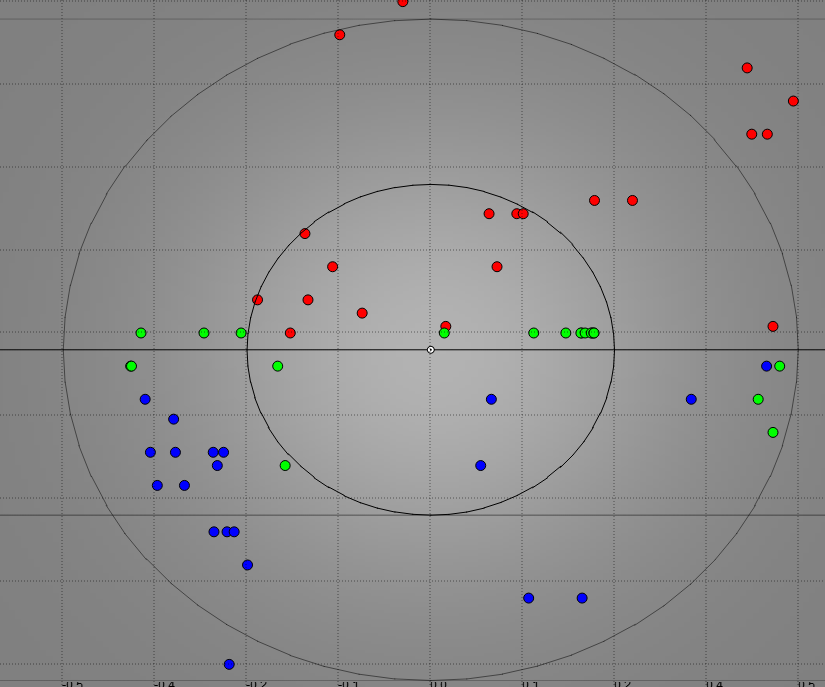
\includegraphics[height=0.11\textheight]{./regression/spheri_kmeans_1_mixture_100train.png}
\caption{\bf Spherical}
\end{subfigure}
\begin{subfigure}[h]{0.3\textwidth}
\centering
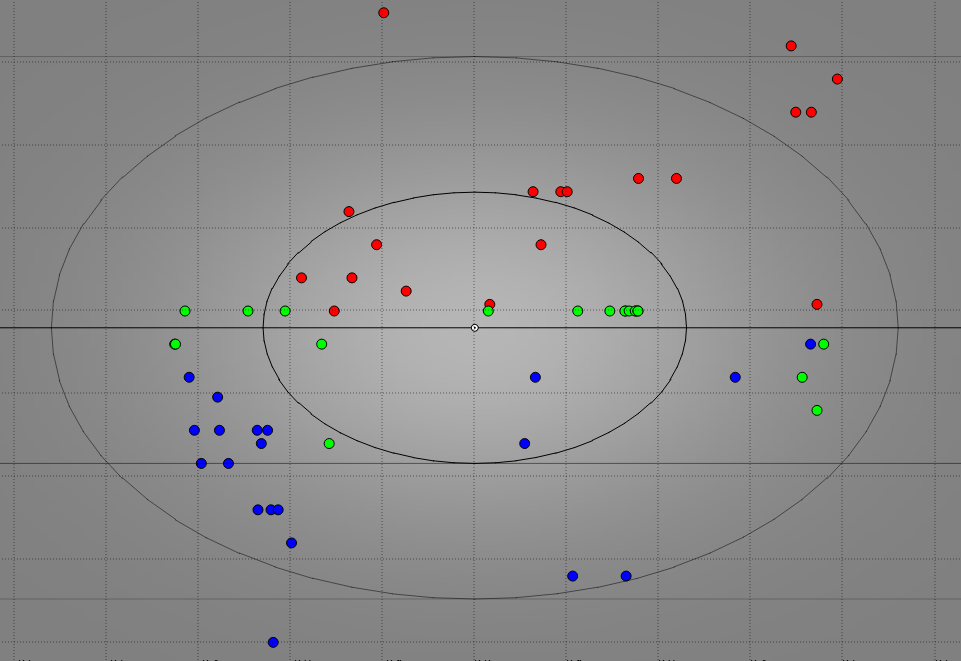
\includegraphics[height=0.11\textheight]{./regression/diag_kmeans_1_mixture_100train.png}
\caption{\bf Diagonal}
\end{subfigure}
\begin{subfigure}[h]{0.3\textwidth}
\centering
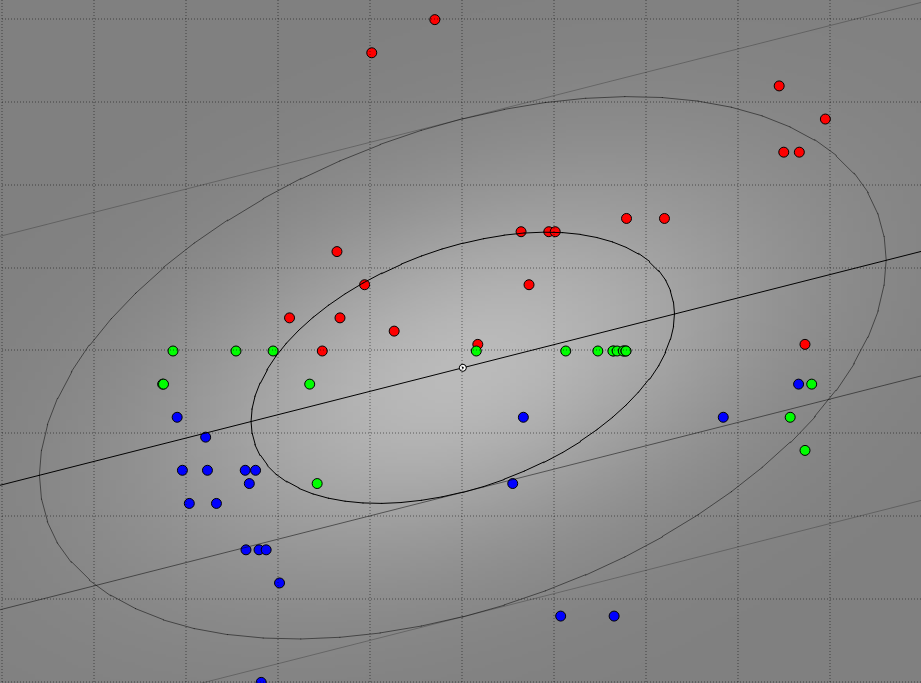
\includegraphics[height=0.11\textheight]{./regression/full_cov_kmeans_1_mixture_100train.png}
\caption{\bf Full}
\end{subfigure}
\caption{GMR : influence of covariance matrix}
\label{fig:covariance_matrix_gmr}
\end{figure}



A spherical and diagonal covariance matrix both give a straight line which represents the mean of the datapoint. In fact, following the regressive signal obtained :
\begin{equation}
y = \sum_{i=1}^K \beta_i(x)(\mu_y^i + \Sigma_{xy}^i (\Sigma_{xx}^i)^{-1}(x - \mu_x^i))  
\label{GMR_output}
\end{equation}
since for spherical and diagonal the quantity, $\Sigma_{xy}^i = 0$, the result is just the mean of the datapoint. 

Then we evaluate the effect of the number of mixture components with a K-means initialization, a full covariance matrix and a training ratio of 100\%. Results are shown on figure \ref{fig:number_mixture_components}.

\begin{figure}[!ht]
\centering
\begin{subfigure}[h]{0.45\textwidth}
\centering
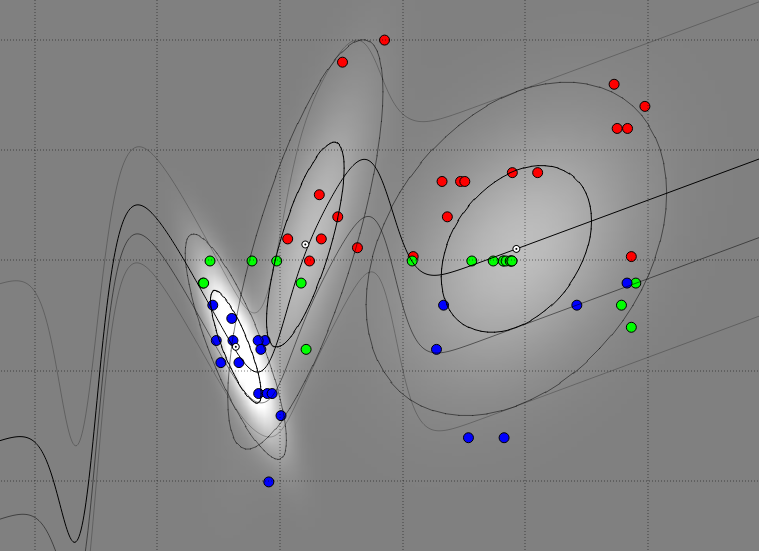
\includegraphics[height=0.11\textheight]{./regression/full_cov_kmeans_3_mixture_100train.png}
\caption{\bf 3 components}
\end{subfigure}
\begin{subfigure}[h]{0.45\textwidth}
\centering
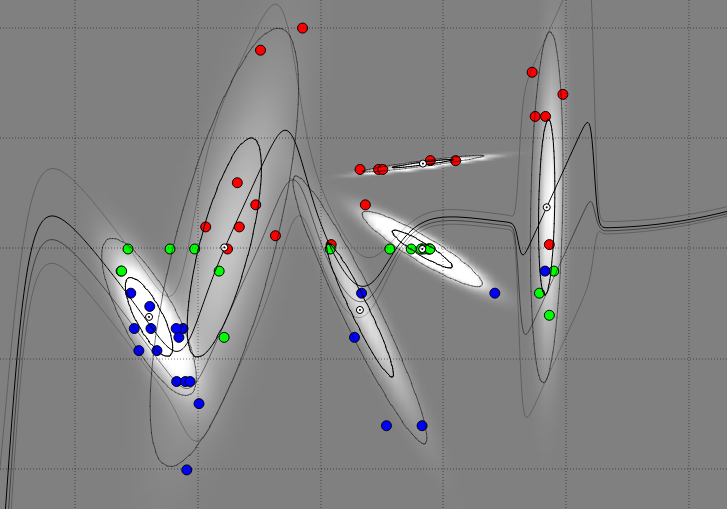
\includegraphics[height=0.11\textheight]{./regression/full_cov_kmeans_6_mixture_100train.png}
\caption{\bf 6 components}
\end{subfigure}

\caption{GMR : influence of number of mixture components}
\label{fig:number_mixture_components}
\end{figure}


With 3 mixture components, there is a poor fit with the large gaussian on the end of the dataset. That is due to the unbalanced number of points in relation to the region and the spread of those points. A solution can be to increase the number of points. In fact, with 6 mixture components, the datapoints are better fitted.

Then, the effect of the initialization is tackled. We used a full covariance matrix and training ratio of 100\%. Results are shown on figure \ref{fig:initialization_gmr}.


\begin{figure}[!ht]
\centering
\begin{subfigure}[h]{0.3\textwidth}
\centering
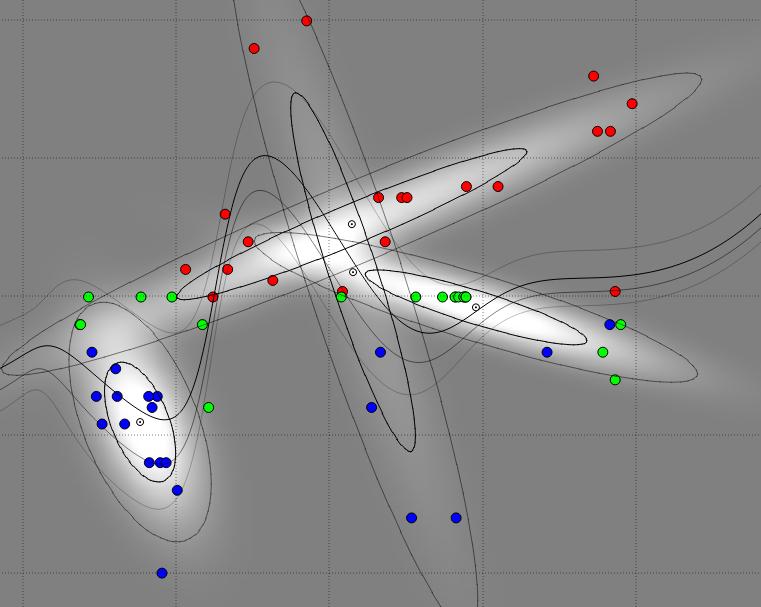
\includegraphics[height=0.11\textheight]{./regression/full_cov_uniform_4_mixture_100train.png}
\caption{\bf Uniform - 4 components}
\end{subfigure}
\begin{subfigure}[h]{0.3\textwidth}
\centering
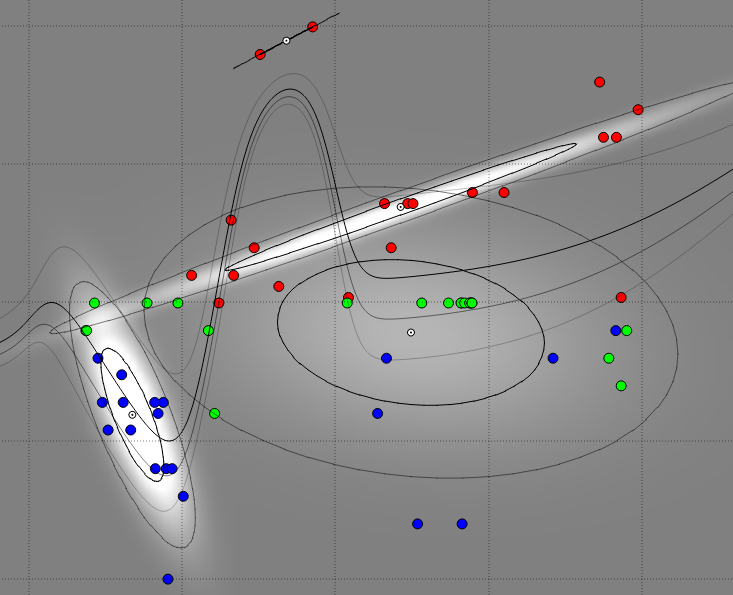
\includegraphics[height=0.11\textheight]{./regression/full_cov_random_4_mixture_100train.png}
\caption{\bf Random - 4 components}
\end{subfigure}
\begin{subfigure}[h]{0.3\textwidth}
\centering
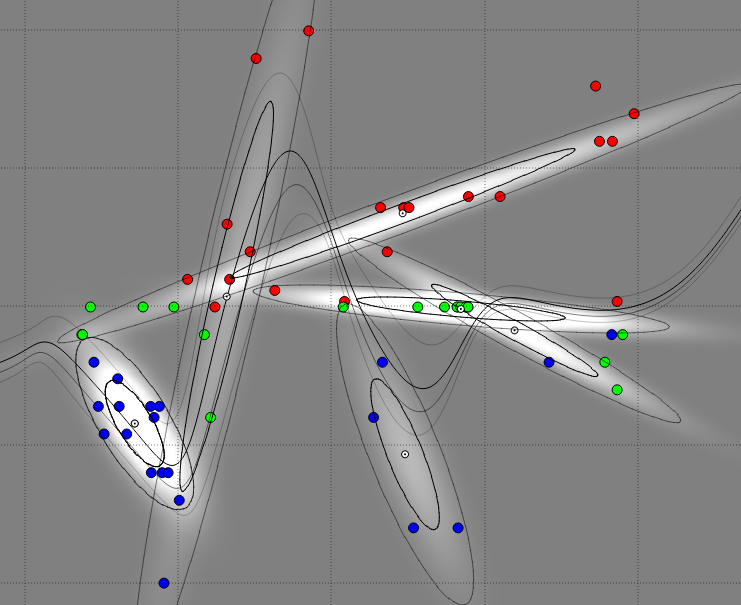
\includegraphics[height=0.11\textheight]{./regression/full_cov_random_7_mixture_100train.png}
\caption{\bf Random - 7 components}
\end{subfigure}
\caption{GMR : influence of initialization}
\label{fig:initialization_gmr}
\end{figure}

We can see that depending on the initialization used, the gaussians fit different points and give different results. For instance with a random initialization and 4 mixture components, in the top, 2 datapoints are fit by one gaussian. Hence, with only 4 mixtures components, the other 3 gaussians can't fit well the datapoint. Hence, we need to increase the number of mixture components which is more costly. Using a uniform or a k-means initialization avoid this situation. 

Then, we change the training ratio using a full covariance matrix and a kmeans initialization. Results are shown on figure \ref{fig:training_ratio_gmr}.


\begin{figure}[!ht]
\centering
\begin{subfigure}[h]{0.3\textwidth}
\centering
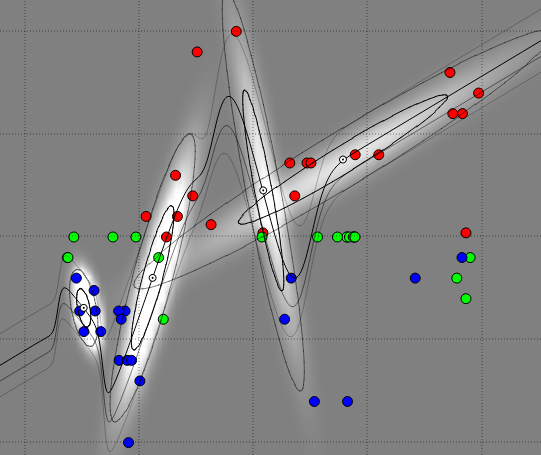
\includegraphics[height=0.11\textheight]{./regression/full_cov_kmeans_4_mixture_33train.png}
\caption{\bf 33\% - 4 components}
\end{subfigure}
\begin{subfigure}[h]{0.3\textwidth}
\centering
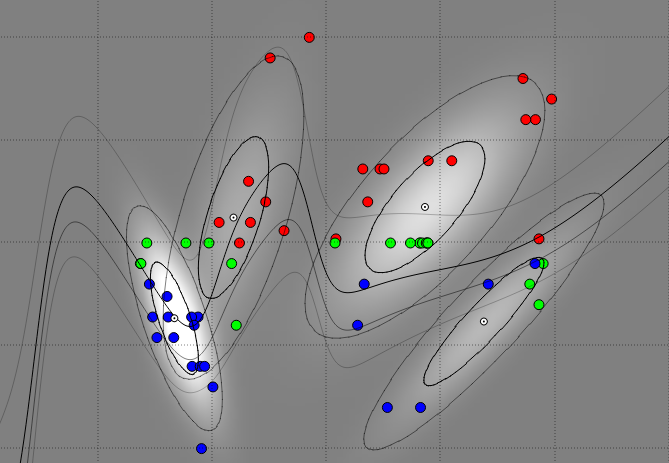
\includegraphics[height=0.11\textheight]{./regression/full_cov_kmeans_4_mixture_66train.png}
\caption{\bf 66\% - 4 components}
\end{subfigure}
\begin{subfigure}[h]{0.3\textwidth}
\centering
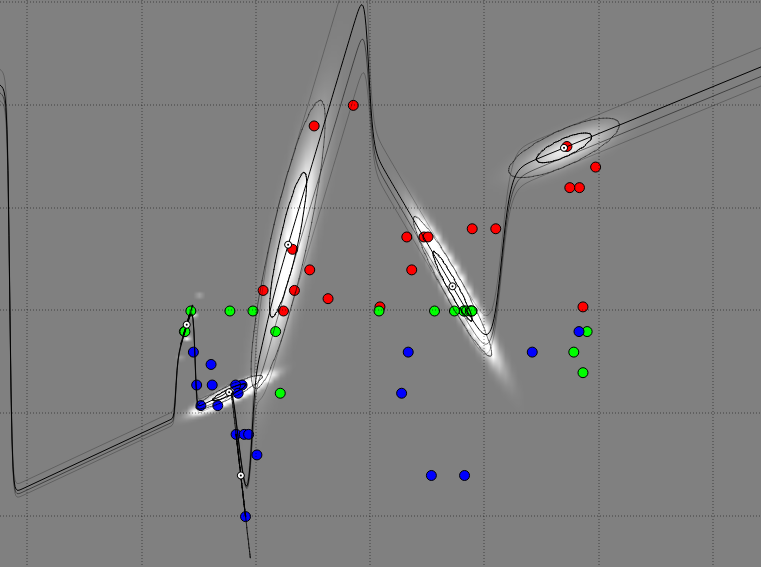
\includegraphics[height=0.11\textheight]{./regression/full_cov_kmeans_6_mixture_33train.png}
\caption{\bf 33\% - 6 components}
\end{subfigure}
\caption{GMR : influence of training ratio}
\label{fig:training_ratio_gmr}
\end{figure}

If we used a too low number of mixture with 33\% of training ratio, the model can missed some points depending on the initialization. To avoid this, we've to enhance the number of datapoint in the training set. As expected with 66\% of training ratio, the model is more able to fit the data. Moreover, we can notice that while increasing the complexity of the model with a larger number of mixture components, with a low training ratio, the model is not able to fit well the datapoints.

\subsubsection{Quantitative evaluation}

In this section, we performed a quantitative evaluation on the all dimensions dataset. We compared different configuration of parameters and looked at the regression error in terms of MSE. We used cross-validation upon 30 folds. Results are shown in figure \ref{fig:quantitative_gmr}.
\begin{figure}[!ht]
\centering
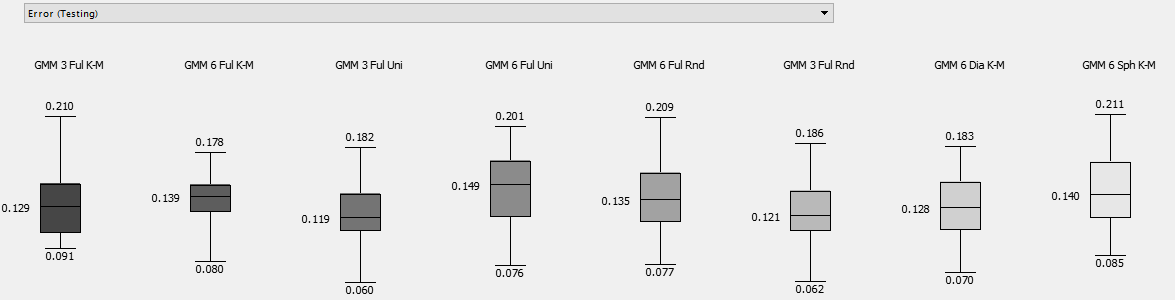
\includegraphics[height=0.15\textheight]{./regression/quantitave_66train_ratio_error_testing.png}
\caption{\bf Error testing - 66\% Training ratio}
\label{fig:quantitative_gmr}
\end{figure}


We have seen that in overall, while increasing the training ratio, the error on testing set decreased a little. Moreover, when we take a look the error for each configuration chosen, it seems that the difference between each model is small. We can also notice the variance is large on the figure for every model meaning that the models are reliable. However, it is very dependent on the initialization as we have seen while running many times.


\subsection{SVR}
% "-SVR: test the RBF kernel; change the kernel degree or width (depending on the kernel);change the penalty factor C (e.g. testing 1-100 or more depending on the range of your output values); change the size of the -tube.
%test the algorithms using different ratios of training/testing samples.
%Run cross-validation on these parameters using the \Compare" window in MLDemos to obtain an estimation of the variance of the results you obtain. Generate graphs and tables of the results you obtain.
Support Vector Machine can also be used as a regression method and keep the main features that characterize the algorithm. The Support Vector Regression (SVR) is a regression method and determine a regressive signal on a subset of the datapoints call support vectors. The output signal is computed with the following formula :
\begin{equation}
y = f(x) = \sum_i \alpha_i k (x^{i},x)
\end{equation}
which $k(x^{i},x)$ represents the kernel function, $\alpha_i$ is a linear coefficient. As we seen on SVM classification section, the algorithm consist of several hyper-parameters. The C-value parameter control the penalty term on poor fit and $\epsilon$ parameter determines the minimal required precision. The predicted output will be in between the \emph{tube} corresponding to $f(x)\pm\epsilon$. 

\subsubsection{Qualitative evaluation}

Firstly, we will perform a regression with a RBF kernel on the 2 dimensional dataset chosen. As we can see on the figure \ref{fig_RBF_0_001_10_0_2_100}
% ADD FIGURE RBF_0.001_10_0.2_100
, the RBF kernel width is small (0.001), thus the kernel places a Gaussian function on each support vectors with a small standard deviation that why the regression overfit the data. Now, if we increase the kernel width (0.3), as shown in the figure \ref{fig_RBF_0_3_10_0_2_100}
% ADD FIGURE RBF_0.3_10_0.2_100
, the  Gaussian function on each support vectors is affected to a higher standard deviation. That means, each support vector will be influenced by the others support vectors neighbor. The resulting regression is smoother than the previous regression.
In order to reduce the effect of the kernel width on the first regression, we reduce the penalty factor C (1.5 comparing to 10) that leads to reduce the overfitting, as we can see on figure \ref{fig_RBF_0_3_1_5_0_2_100}.
% ADD FIGURE RBF_0.3_1.5_0.2_100
If we reduce the size of the $\epsilon-tube$ (0.05 comparing to 0.2 for the previous regression), the resulting regression, on figure \ref{fig_RBF_0_001_5_0_05_100}, will overfit the data. 
% ADD FIGURE RBF_0.001_5_0.05_100

% With Train test ration : 33%
Then, we decrease the train test ratio to 33\%, the figure \ref{fig_RBF_0_001_10_0_15_33} show the obtained regression. We observe the number of support vector decrease and depend on the initialization.
% ADD FIGURE RBF_0.001_10_0.15_33

\begin{figure}[!ht]
\centering
\begin{subfigure}[h]{0.3\textwidth}
\centering
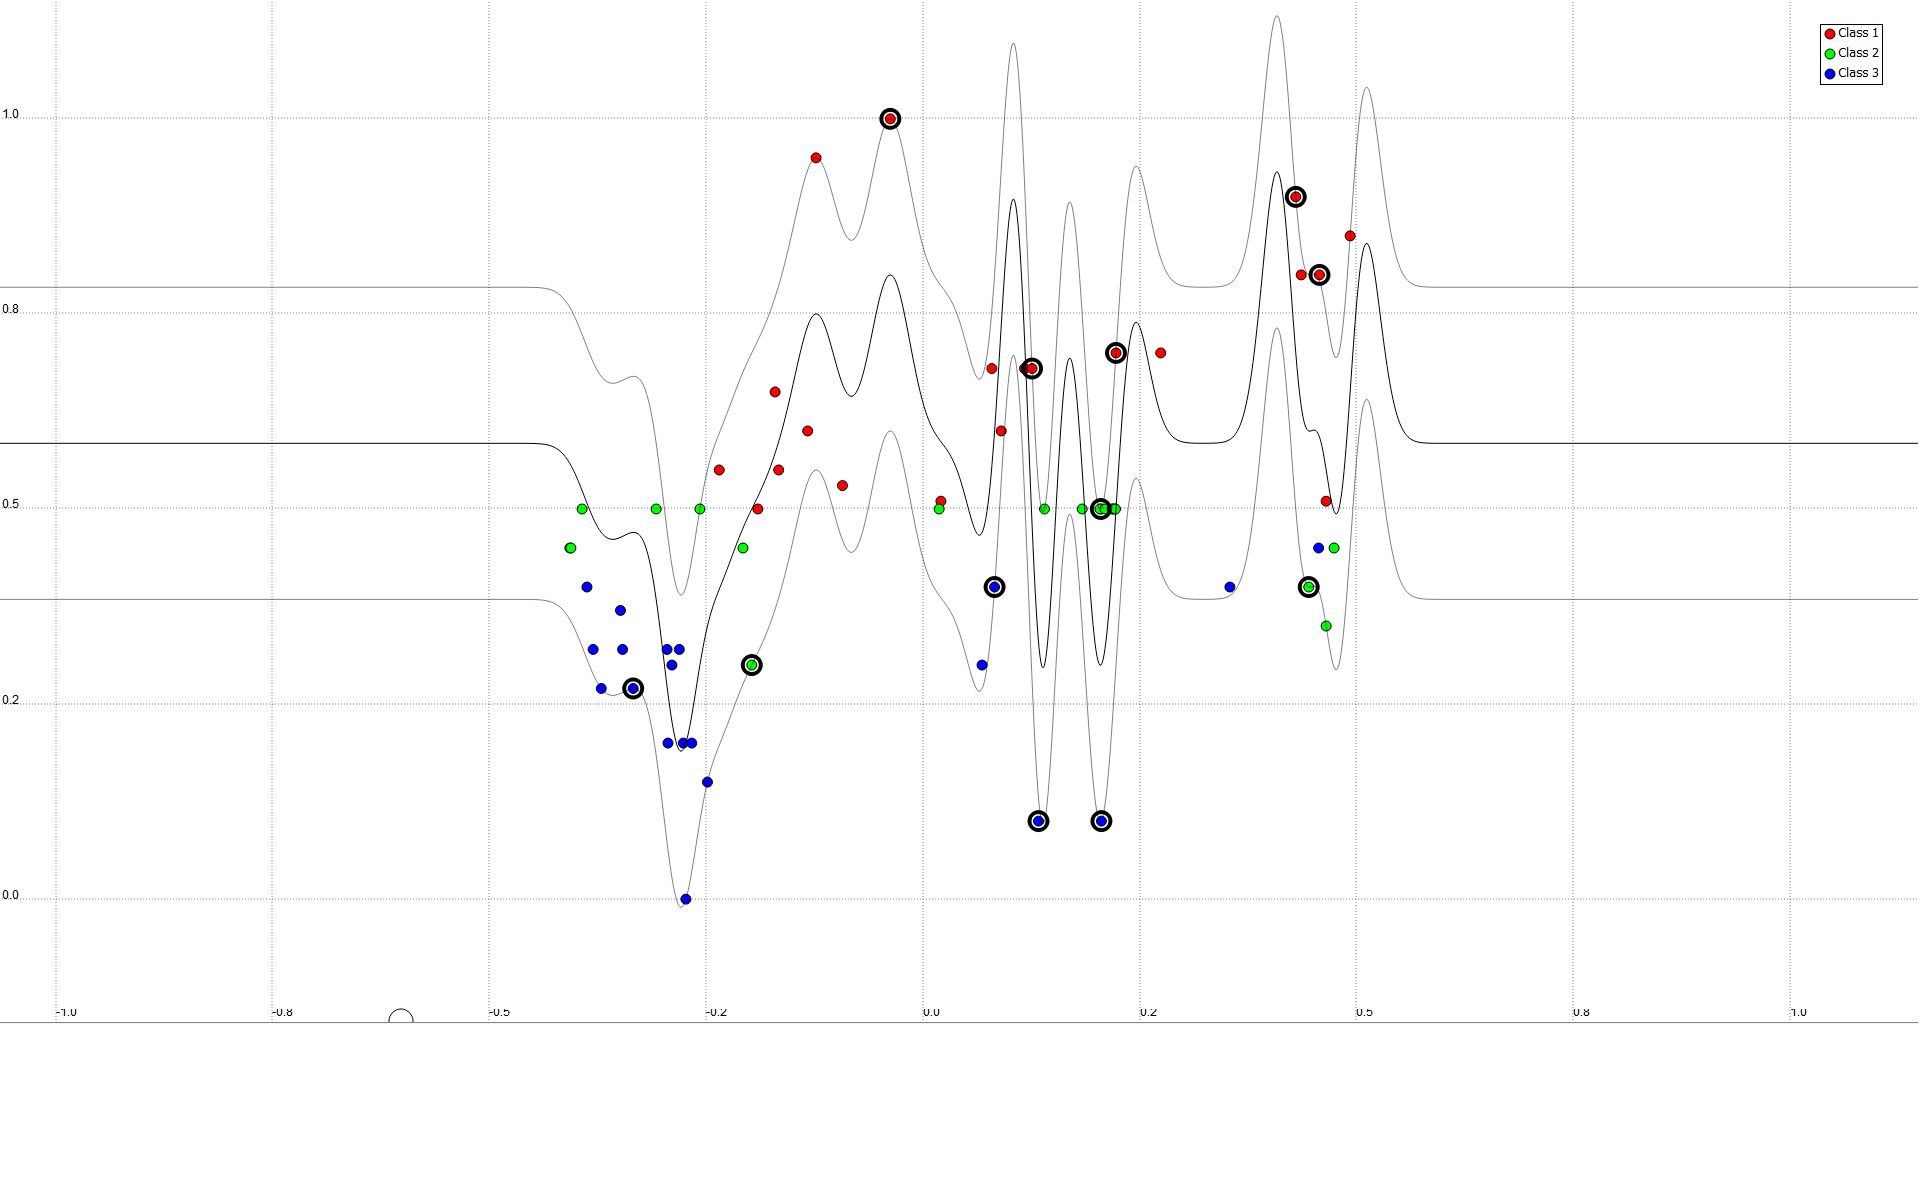
\includegraphics[height=0.11\textheight]{./regression/RBF_0_001_10_0_2_100.png}
\caption{\bf kernel : 0.001, C-value:10, $\epsilon-tube$ : 0.2, TR: 100\%}
\label{fig_RBF_0_001_10_0_2_100}
\end{subfigure}
\begin{subfigure}[h]{0.3\textwidth}
\centering
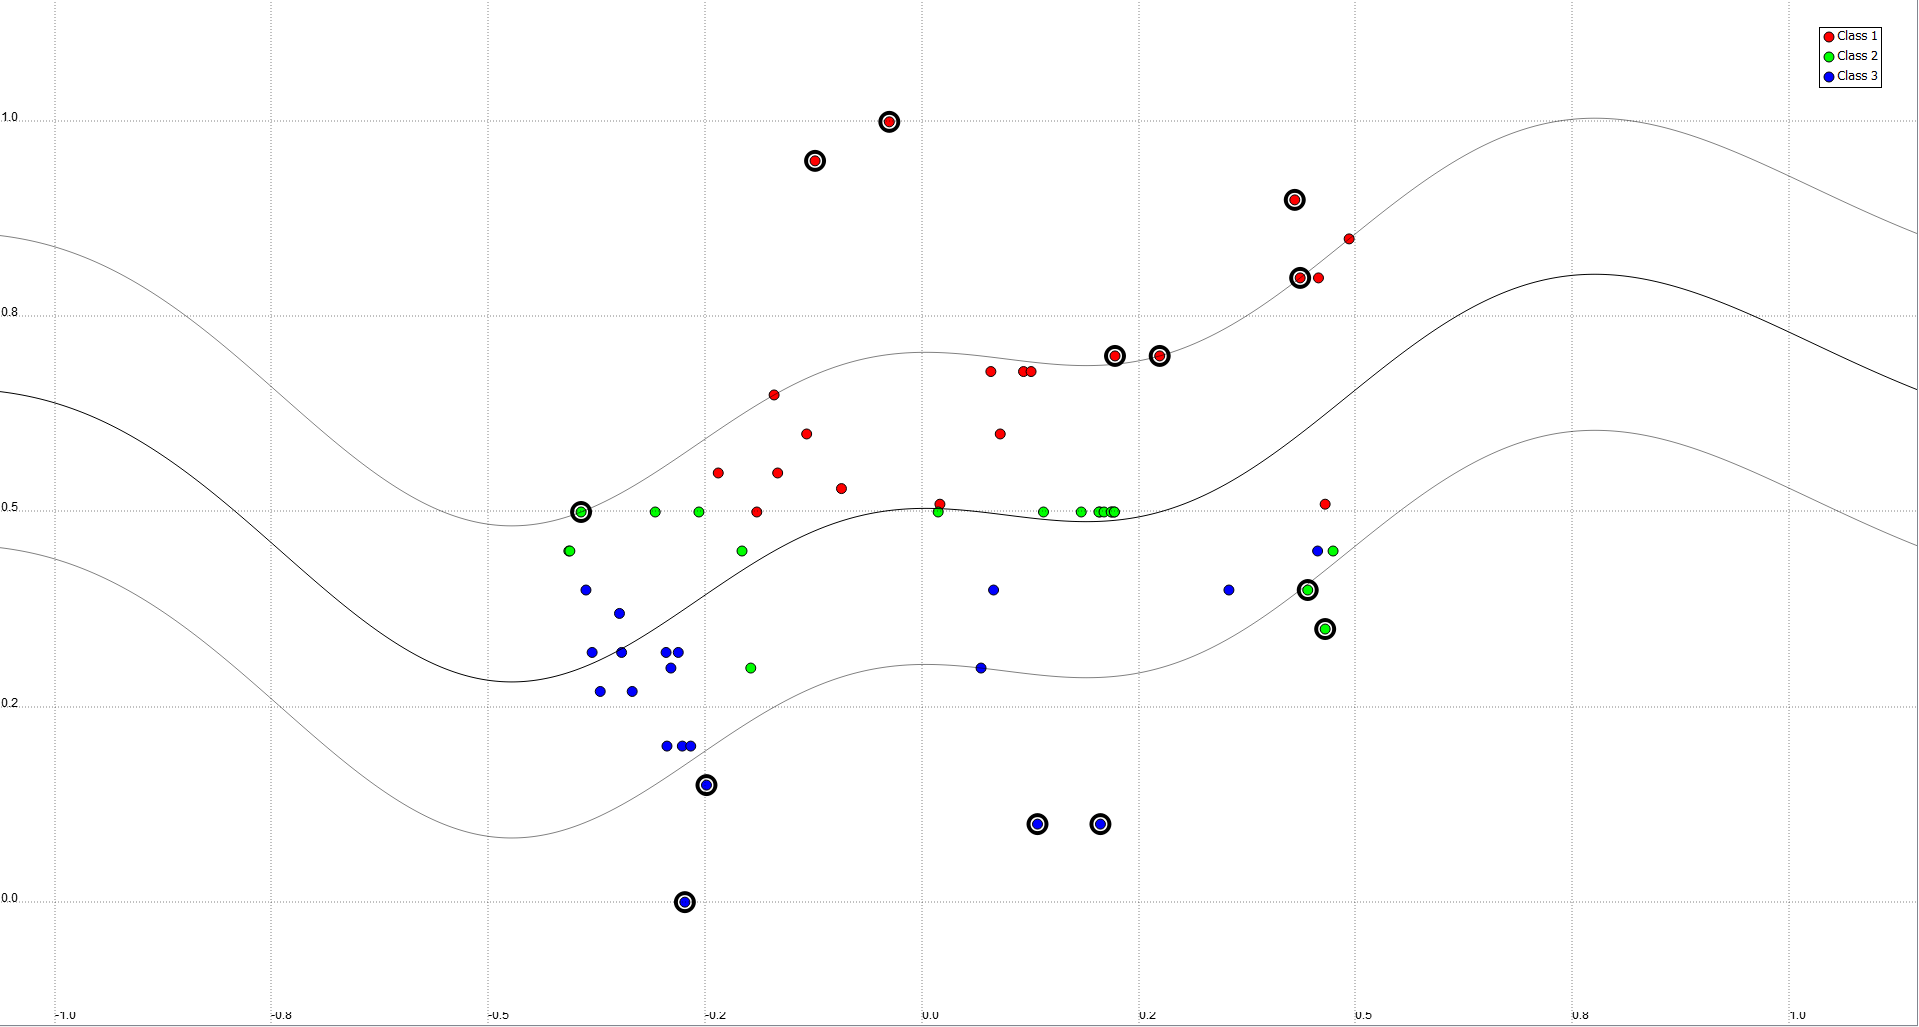
\includegraphics[height=0.11\textheight]{./regression/RBF_0_3_10_0_2_100.png}
\caption{\bf kernel : 0.3, C-value:10, $\epsilon-tube$ : 0.2, TR: 100\%}
\label{fig_RBF_0_3_10_0_2_100}
\end{subfigure}
\begin{subfigure}[h]{0.3\textwidth}
\centering
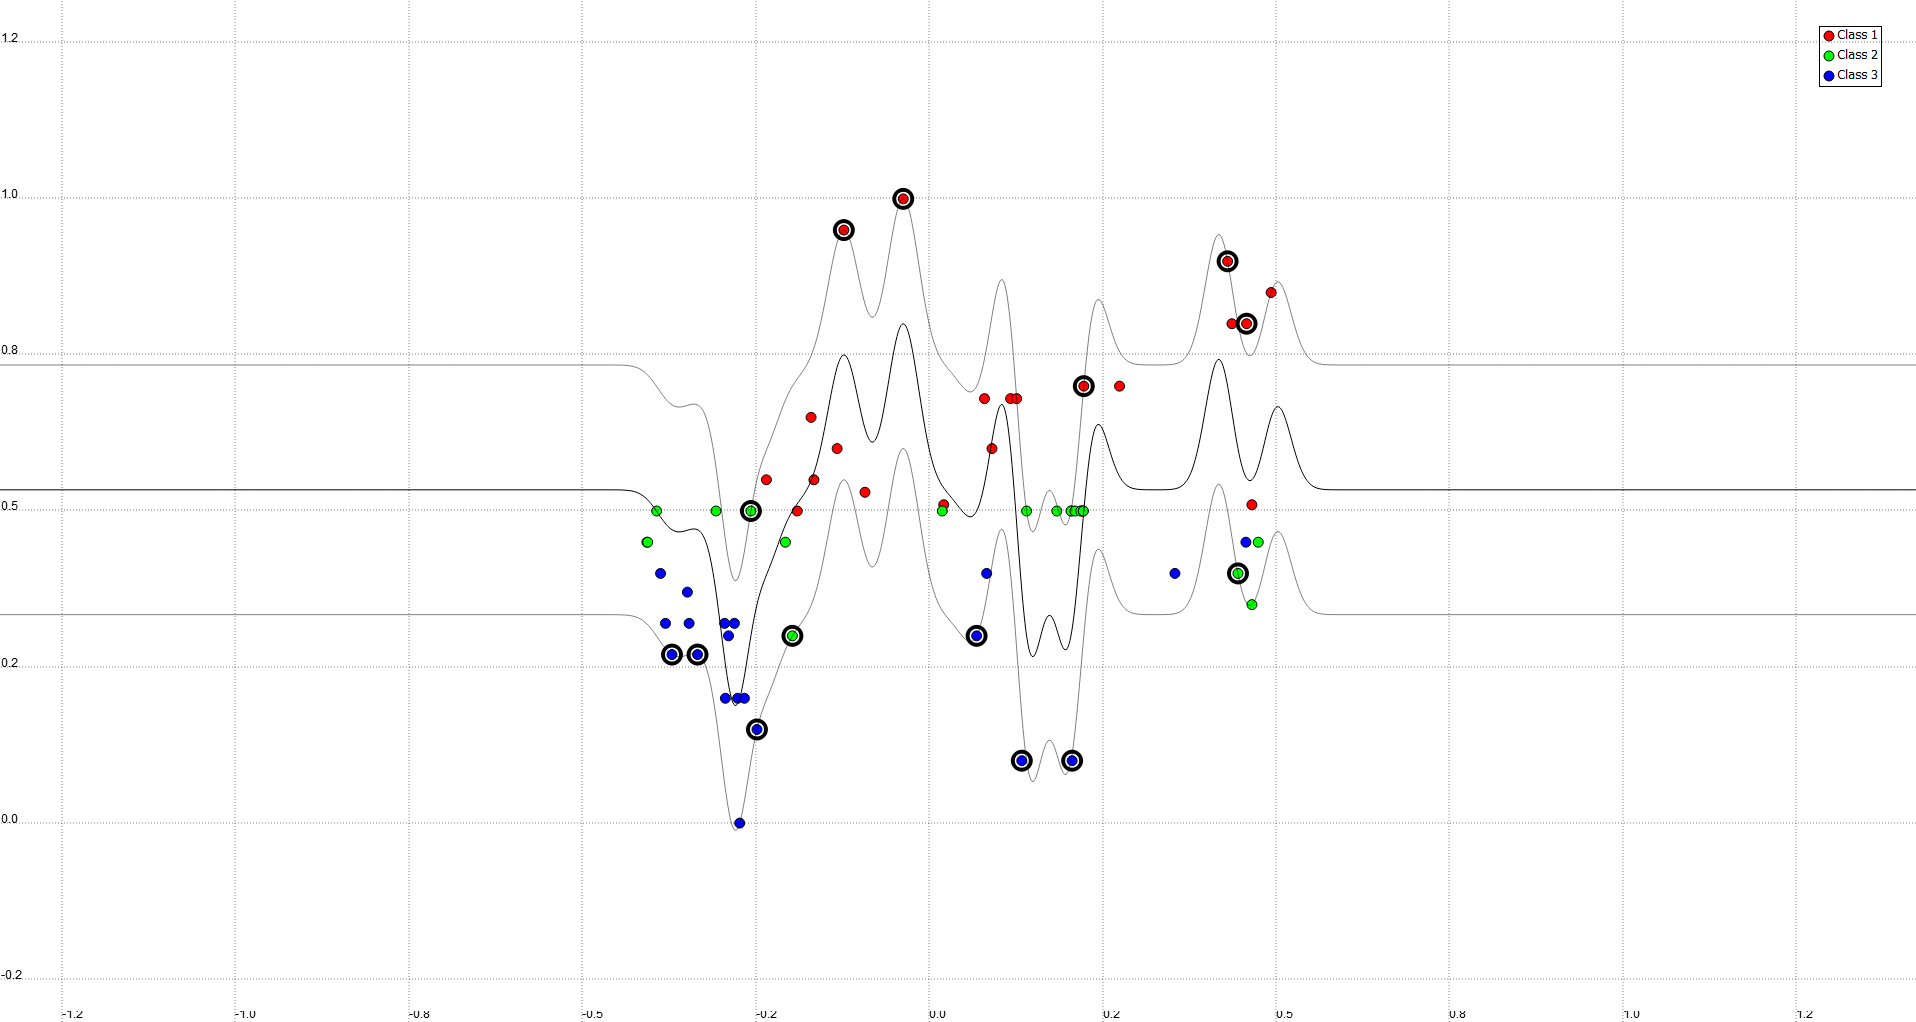
\includegraphics[height=0.11\textheight]{./regression/RBF_0_3_1_5_0_2_100.png}
\caption{\bf kernel : 0.3, C-value:1.5, $\epsilon-tube$ : 0.2, TR: 100\%}
\label{fig_RBF_0_3_1_5_0_2_100}
\end{subfigure}
\begin{subfigure}[h]{0.3\textwidth}
\centering
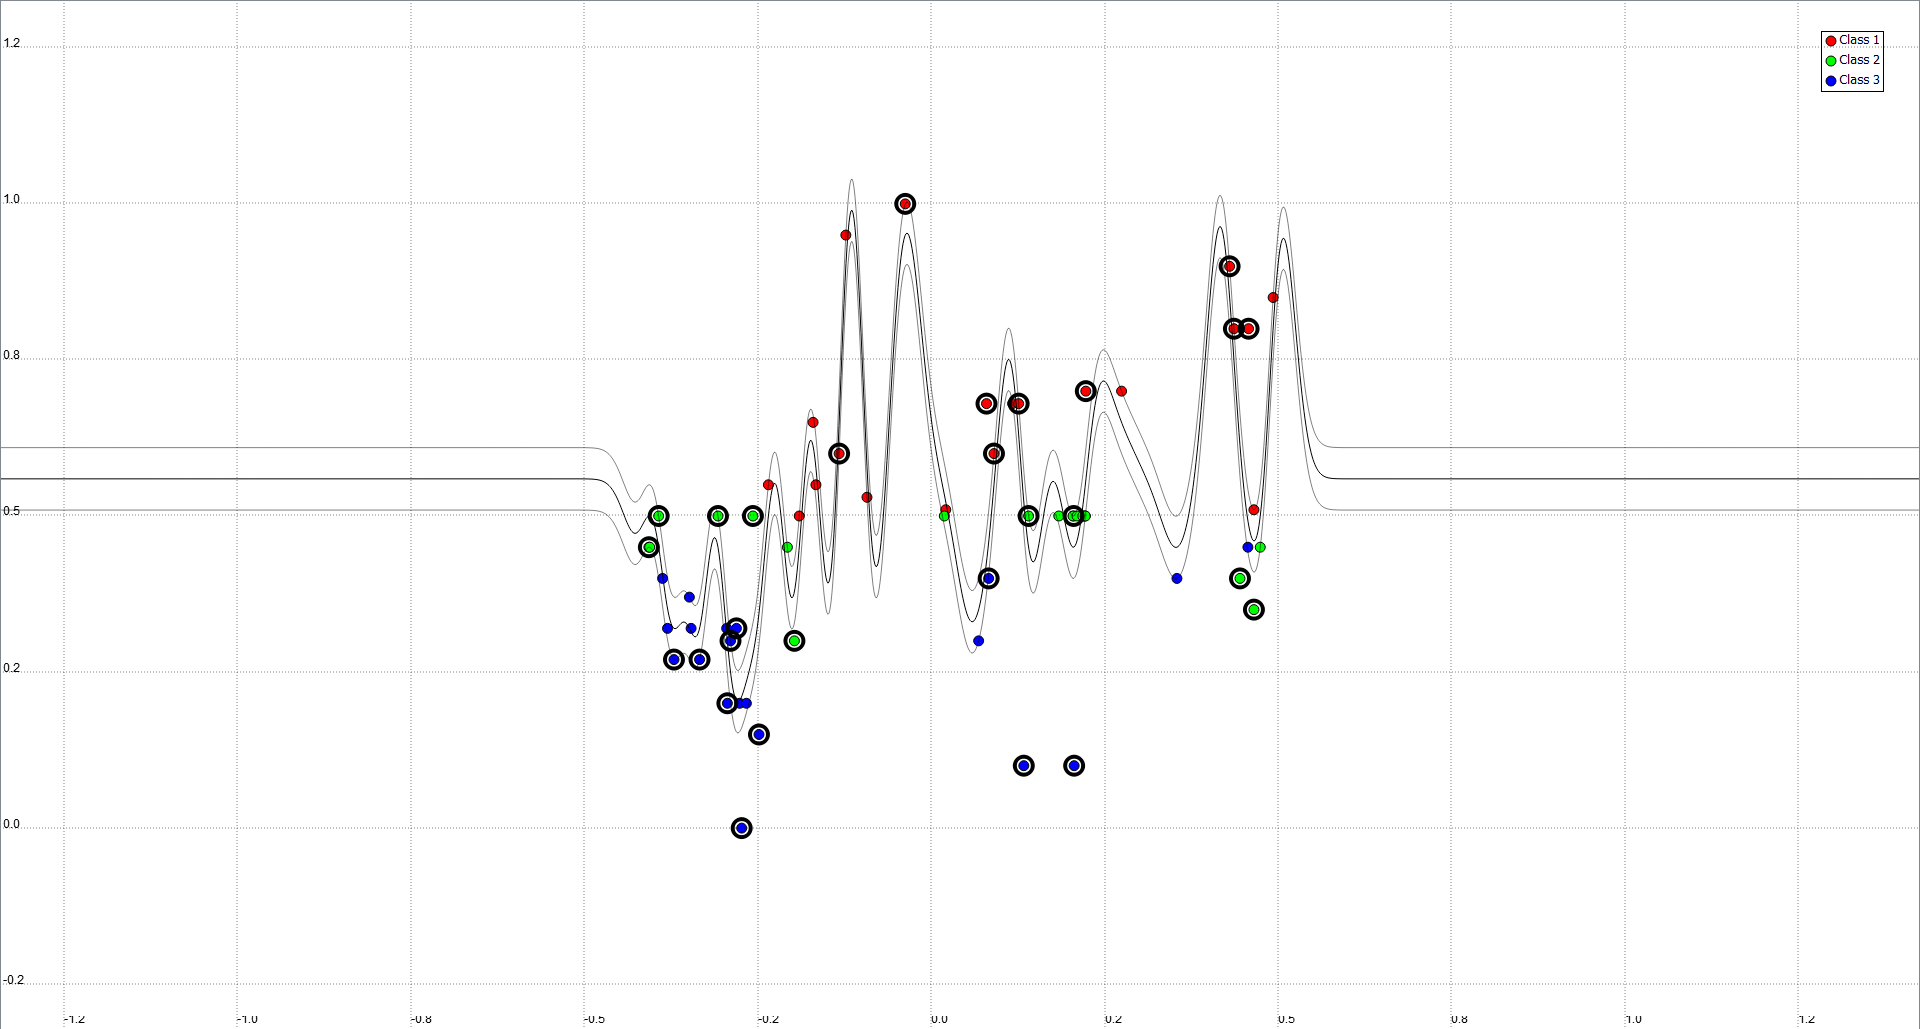
\includegraphics[height=0.11\textheight]{./regression/RBF_0_001_5_0_05_100.png}
\caption{\bf kernel : 0.001, C-value:5, $\epsilon-tube$ : 0.05, TR: 100\%}
\label{fig_RBF_0_001_5_0_05_100}
\end{subfigure}
\begin{subfigure}[h]{0.3\textwidth}
\centering
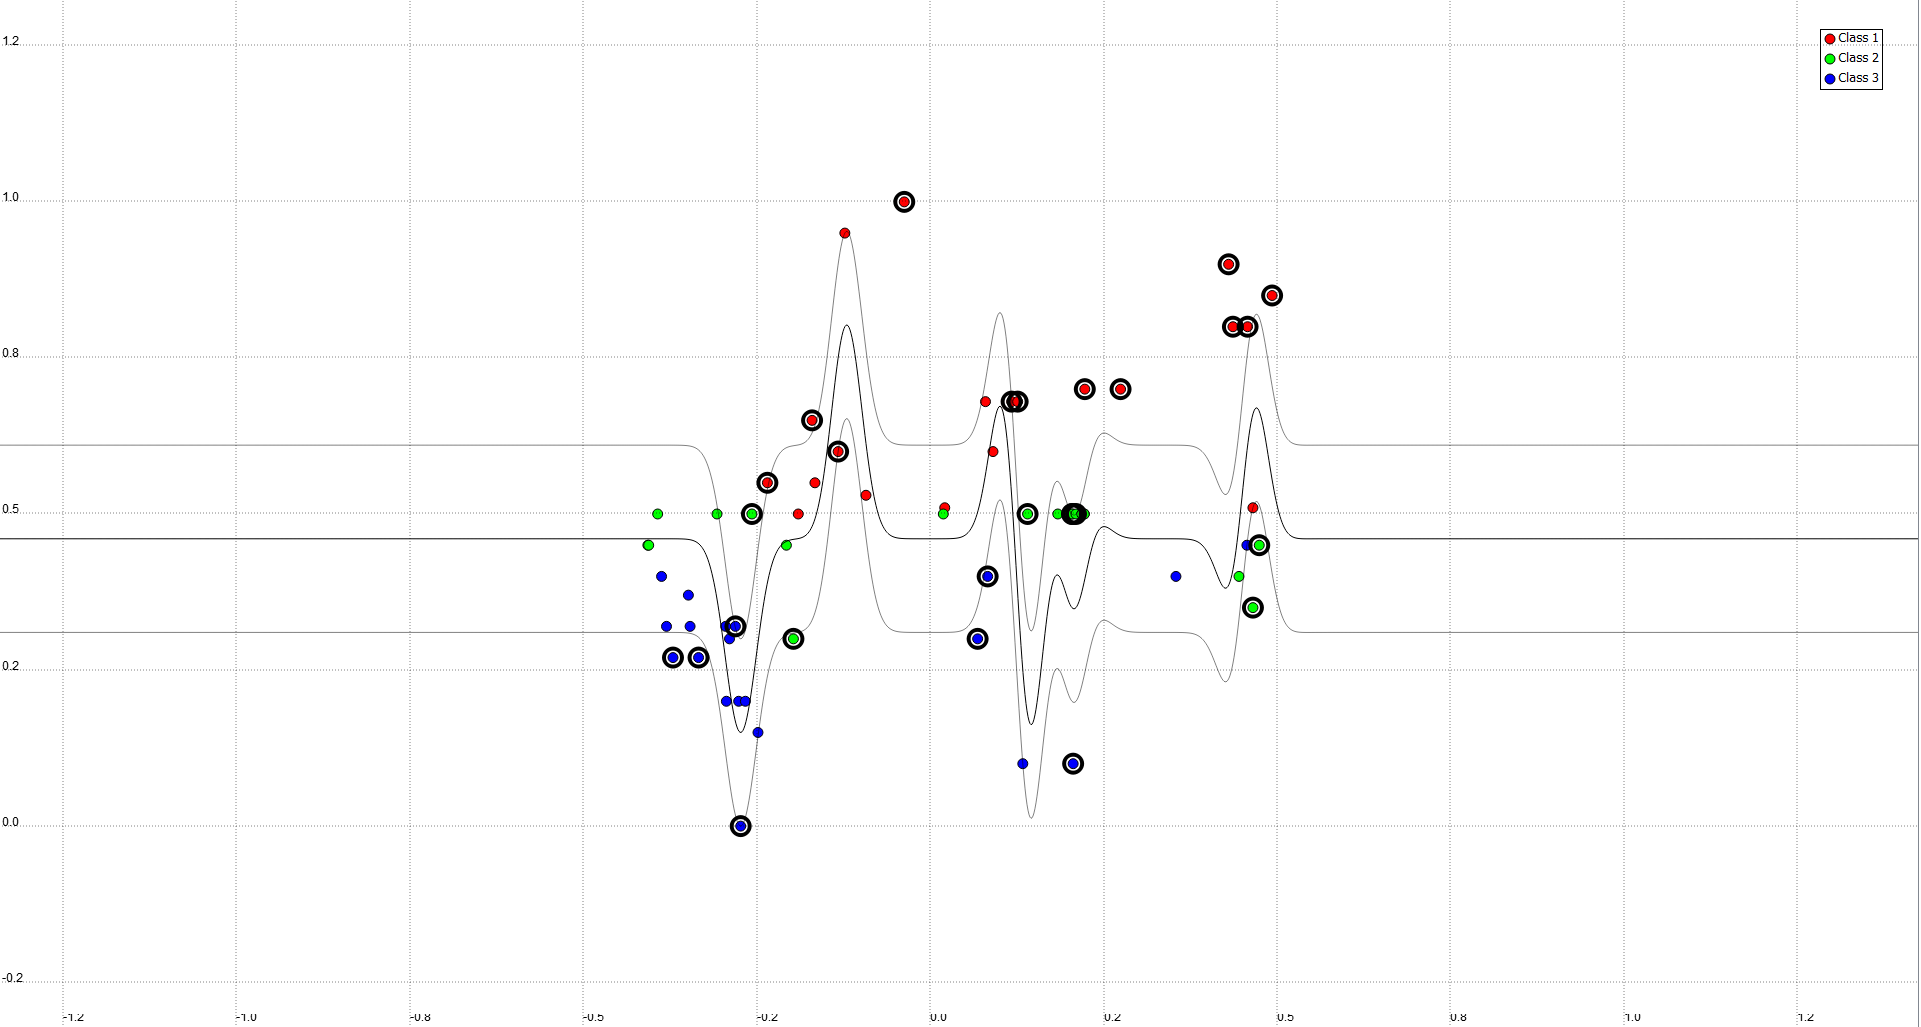
\includegraphics[height=0.11\textheight]{./regression/RBF_0_001_10_0_15_33.png}
\caption{\bf kernel : 0.001, C-value:10, $\epsilon-tube$ : 0.15, TR: 33\%}
\label{fig_RBF_0_001_10_0_15_33}
\end{subfigure}

\caption{SVR : influence of differents parameters}
\end{figure}


\subsubsection{Quantitative evaluation}

We performed several regression with different hyper parameters on the (N+1) dimensions dataset, then we compare the performance of the resulting regression in terms of Mean Square Error. 
As shown on the figure \ref{fig:quantitative_svr}, the configuration which has the less error is one with the small kernel width. However, the algorithm with higher $\epsilon-tube$ has the a small variance and a larger error, that means the regression is reliable.
% ADD MSE qualitative 66
\begin{figure}[!ht]
\centering
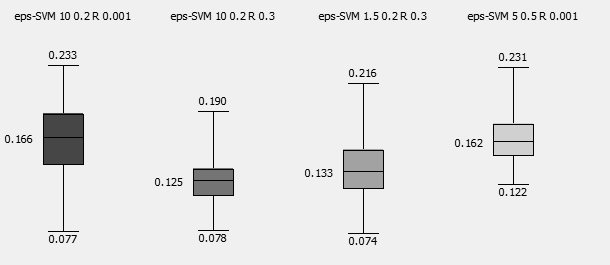
\includegraphics[height=0.15\textheight]{./regression/MSE_quantitative_66.png}
\caption{\bf Error testing - 66\% Training ratio}
\label{fig:quantitative_svr}
\end{figure}
